% \appendix
% 📚 appendix_ch6_massive_mimo_mmwave.tex

\chapter{Chapter 6 – Massive MIMO \& mmWave}

\section{Appendix: Chapter 6 – Massive MIMO \& mmWave}
\addcontentsline{toc}{section}{Appendix: Chapter 6 – Massive MIMO \& mmWave}

\subsection{Notebook: \texttt{A6\_massive\_mimo\_mmwave.ipynb}}

This notebook provides simulations and visualizations for the concepts of Massive MIMO and millimeter-wave (mmWave) communication. It covers:

\begin{itemize}
    \item Simulation of MIMO channel capacity vs number of antennas
    \item Path loss modeling at mmWave frequencies (e.g., 28 GHz, 60 GHz)
    \item Beamwidth estimation as a function of antenna array size
    \item Exploration of high-frequency signal propagation characteristics
\end{itemize}

\subsection{Figures}

\begin{figure}[H]
    \centering
    \includegraphics[width=0.85\textwidth]{figures/massive_mimo_capacity_plot.png}
    \caption{Channel capacity vs number of receive antennas (Massive MIMO)}
\end{figure}

\begin{figure}[H]
    \centering
    \includegraphics[width=0.85\textwidth]{figures/mmwave_path_loss_plot.png}
    \caption{Path loss at 2.4, 28, and 60 GHz over distance (mmWave)}
\end{figure}

\begin{figure}[H]
    \centering
    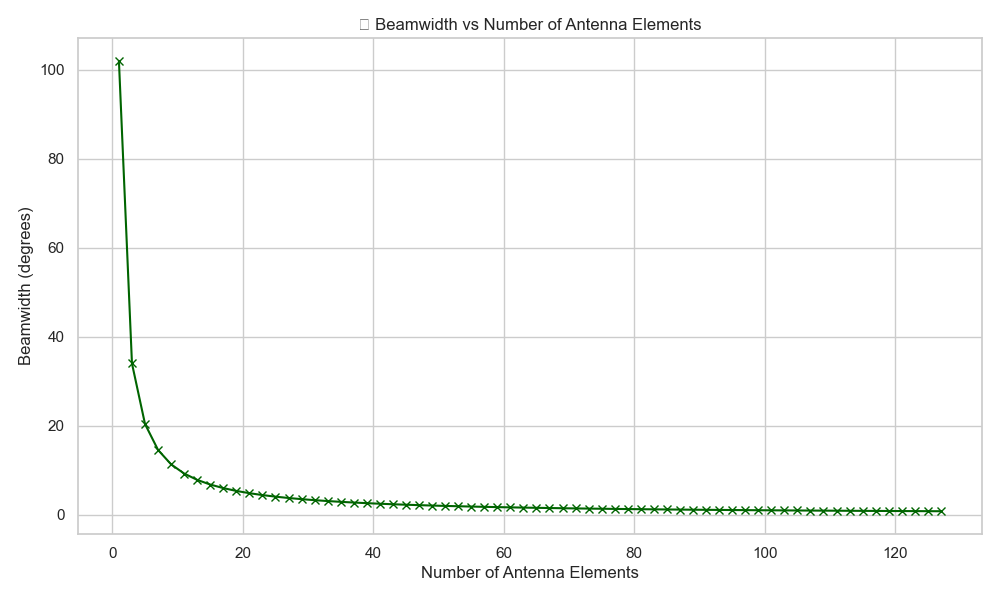
\includegraphics[width=0.75\textwidth]{figures/beamwidth_vs_elements.png}
    \caption{Beamwidth vs number of antenna elements}
\end{figure}

\subsection{Optional Streamlit App: \texttt{MassiveMIMODemo.py}}

An interactive companion to the notebook is provided in the form of a Streamlit app with the following features:

\begin{itemize}
    \item Real-time capacity simulations as a function of $N_t$, $N_r$, and SNR
    \item Toggleable path loss curves for different mmWave frequencies
    \item Visualization of beamwidth narrowing with increasing antenna count
\end{itemize}

\textbf{Location:} \texttt{pages/MassiveMIMODemo.py}

\subsection*{References}
\begin{itemize}
    \item T. L. Marzetta, “Noncooperative cellular wireless with unlimited numbers of base station antennas,” IEEE Transactions on Wireless Communications, 2010.
    \item R. Heath et al., “An Overview of Signal Processing Techniques for Millimeter Wave MIMO Systems,” IEEE Journal of Selected Topics in Signal Processing, 2016.
    \item 3GPP TR 38.900: Study on channel model for frequencies from 0.5 to 100 GHz.
\end{itemize}



\section{Appendix: Massive MIMO and mmWave Simulation}

This appendix complements Chapter 6 by providing simulation results and visualization for concepts in Massive MIMO and mmWave communications. The figures included were generated via the companion Jupyter notebook \texttt{A6\_massive\_mimo\_mmwave.ipynb}.

\subsection{Massive MIMO Capacity Scaling}

The figure below shows how the MIMO channel capacity increases with the number of receive antennas for a fixed number of transmit antennas and fixed SNR. This illustrates the spatial multiplexing gain that becomes significant in Massive MIMO systems.

\begin{figure}[h]
    \centering
    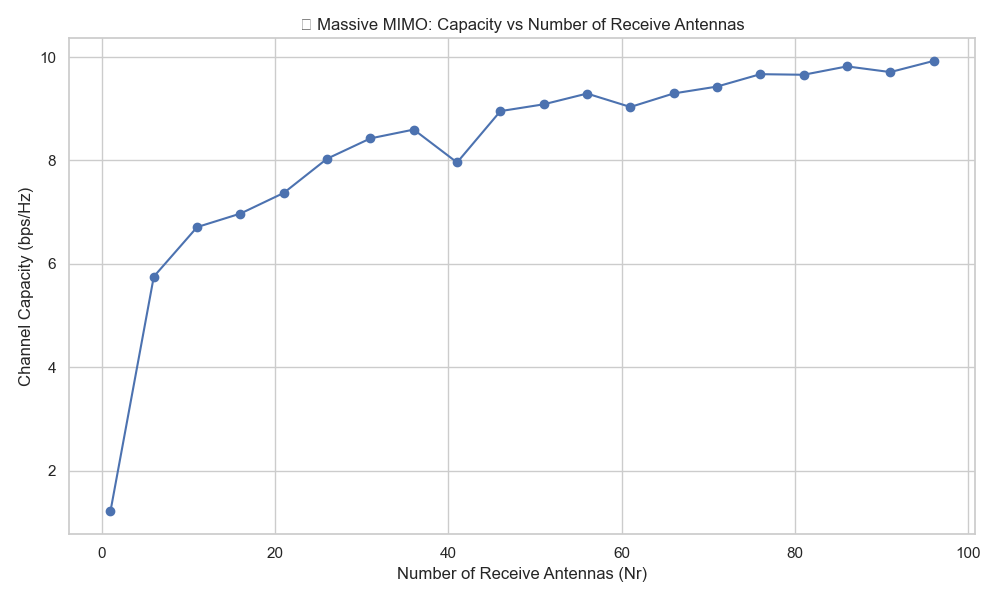
\includegraphics[width=0.85\textwidth]{figures/massive_mimo_capacity.png}
    \caption{Channel Capacity vs. Number of Receive Antennas for MIMO}
    \label{fig:mimo_capacity}
\end{figure}

\subsection{Beamwidth Reduction with Antenna Array Size}

This simulation demonstrates how beamwidth narrows with an increasing number of antenna elements in a uniform linear array (ULA). Narrower beams enable better spatial selectivity and interference rejection.

\begin{figure}[h]
    \centering
    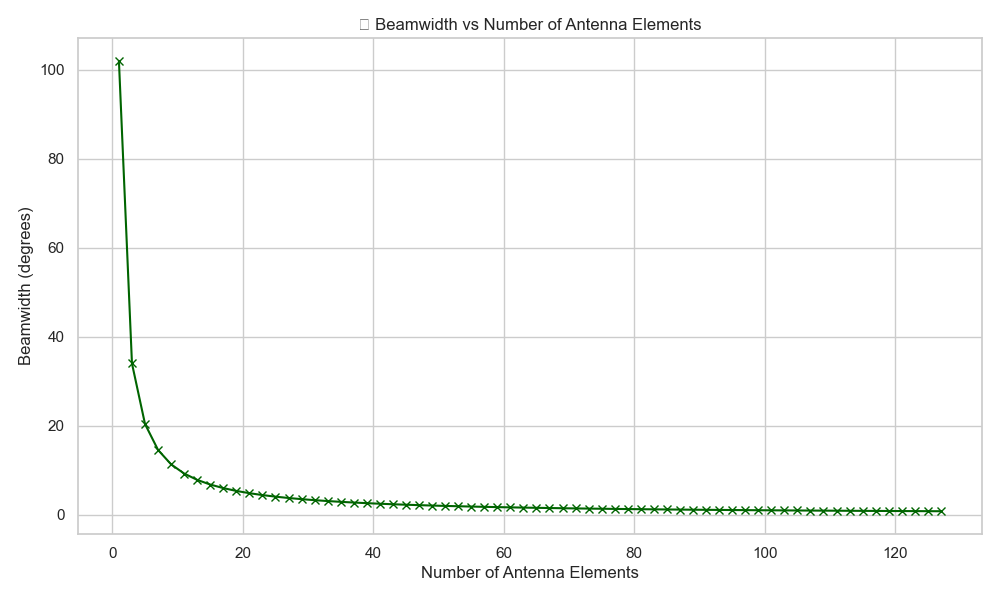
\includegraphics[width=0.75\textwidth]{figures/beamwidth_vs_elements.png}
    \caption{Beamwidth vs. Number of Antenna Elements}
    \label{fig:beamwidth_vs_elements}
\end{figure}

\subsection{Free-Space Path Loss Across mmWave Frequencies}

As frequency increases, so does the free-space path loss (FSPL). The figure below compares FSPL at 2.4 GHz (sub-6 GHz), 28 GHz, and 60 GHz (mmWave band) across a distance range from 1 to 1000 meters.

\begin{figure}[h]
    \centering
    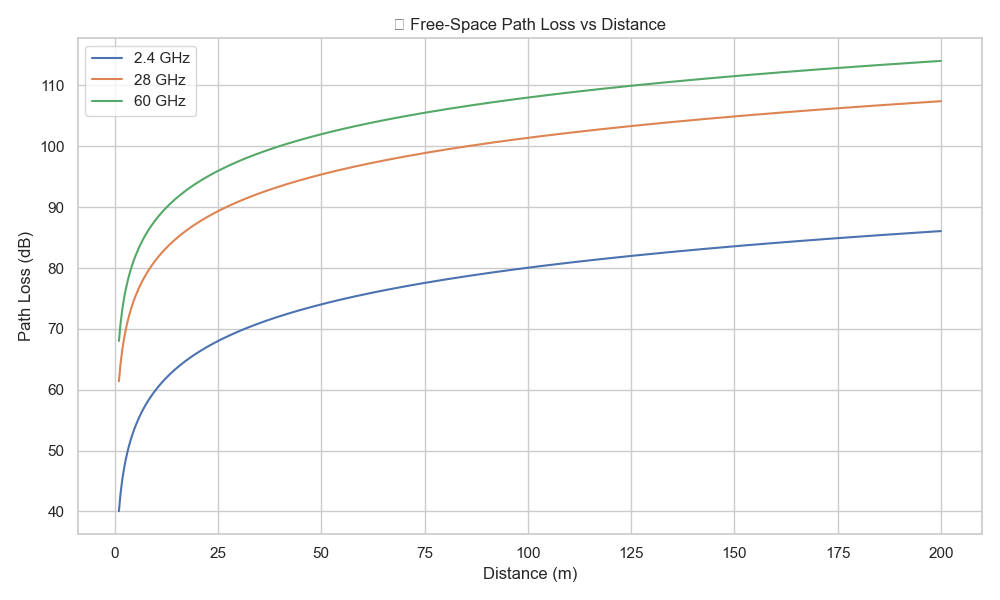
\includegraphics[width=0.85\textwidth]{figures/mmwave_fspl_comparison.png}
    \caption{FSPL Comparison at 2.4 GHz, 28 GHz, and 60 GHz}
    \label{fig:mmwave_fspl}
\end{figure}

\subsection{Notebook and App Reference}

You may explore these simulations interactively using the following resources:

\begin{itemize}
    \item \textbf{Notebook:} \texttt{A6\_massive\_mimo\_mmwave.ipynb}
    \item \textbf{Streamlit App:} \texttt{MassiveMIMODemo.py} (see page \textit{Massive MIMO Demo} in the simulation dashboard)
\end{itemize}

\subsection{Further Reading}

\begin{itemize}
    \item T. L. Marzetta, “Noncooperative cellular wireless with unlimited numbers of base station antennas,” IEEE Trans. Wireless Commun., 2010.
    \item R. W. Heath Jr., N. González-Prelcic et al., “An Overview of Signal Processing Techniques for Millimeter Wave MIMO Systems,” IEEE J. Sel. Top. Signal Process., 2016.
    \item S. Rangan, T. S. Rappaport, and E. Erkip, “Millimeter-wave cellular wireless networks: Potentials and challenges,” Proc. IEEE, 2014.
\end{itemize}

